\documentclass[UTF8,twocolumn,10pt,a4paper]{ctexart}

\usepackage[a4paper,left=1.55cm,right=1.55cm,top=1.45cm,bottom=1.60cm,columnsep=0.66cm]{geometry}
\usepackage{fontspec}
\setmainfont{DejaVu Serif}
\setsansfont{DejaVu Sans}
\setmonofont{DejaVu Sans Mono}
\IfFontExistsTF{Noto Serif CJK SC}{\setCJKmainfont{Noto Serif CJK SC}}{}
\IfFontExistsTF{Noto Sans CJK SC}{\setCJKsansfont{Noto Sans CJK SC}}{}
\IfFontExistsTF{Noto Sans Mono CJK SC}{\setCJKmonofont{Noto Sans Mono CJK SC}}{}

\usepackage{amsmath,amssymb,mathtools,bm}
\usepackage{booktabs,tabularx,array,multirow}
\usepackage{graphicx}
\usepackage{enumitem}
\usepackage{microtype}
\usepackage{xcolor}
\usepackage[hidelinks]{hyperref}

\hypersetup{
  pdftitle={TGVF Representation Phase: Method and Preliminary Grounding Validation},
  pdfauthor={TGVF Project},
  pdfsubject={Implementation-grounded report for target-specific readable visual representations},
  pdfkeywords={TGVF, representation learning, Matrix CE, DeepStack, grounding, hallucination}
}

\graphicspath{{figures/}}
\setlength{\parindent}{1em}
\setlength{\parskip}{0.12em}
\renewcommand{\baselinestretch}{1.015}
\setlength{\abovedisplayskip}{4.4pt plus 1pt minus 1pt}
\setlength{\belowdisplayskip}{4.4pt plus 1pt minus 1pt}
\setlength{\abovedisplayshortskip}{2.4pt plus 1pt}
\setlength{\belowdisplayshortskip}{2.4pt plus 1pt minus 1pt}
\setlength{\textfloatsep}{7pt plus 2pt minus 2pt}
\setlength{\dbltextfloatsep}{7pt plus 2pt minus 2pt}
\setlength{\intextsep}{6pt plus 2pt minus 2pt}
\setlength{\emergencystretch}{1.5em}
\ctexset{
  section={beforeskip=0.72ex plus .2ex,afterskip=0.34ex plus .1ex,format=\large\bfseries},
  subsection={beforeskip=0.58ex plus .2ex,afterskip=0.26ex plus .1ex,format=\normalsize\bfseries},
  paragraph={beforeskip=0.45ex plus .15ex,afterskip=0.55em,runin=true,format=\normalsize\bfseries}
}
\setlist{nosep,leftmargin=1.45em}
\allowdisplaybreaks

\newcolumntype{Y}{>{\raggedright\arraybackslash}X}
\newcommand{\softmax}{\operatorname{softmax}}
\newcommand{\LN}{\operatorname{LN}}
\newcommand{\TGVF}{\textsf{TGVF}}
\newcommand{\DMain}{D^{(0)}}
\newcommand{\DDS}{\{D^{(8)},D^{(16)},D^{(24)}\}}
\newcommand{\code}[1]{\texttt{#1}}

\title{\vspace{-1.0em}\textbf{TGVF Representation Phase：\newline
原生工具条件下的目标特异视觉表征与初步 Grounding 验证}}
\author{TGVF Project}
\date{实现与验证报告，2026 年 7 月 21 日}

\begin{document}
\maketitle
\vspace{-1.55em}

\begin{abstract}
本文报告 TGVF 新管线中的 representation phase（历史项目中曾称 Stage1）的当前方法、训练实现与验证证据。该阶段不训练回答策略，而是在冻结 Qwen3-VL-8B-Thinking 的条件下，仅训练 TGVF Adapter，使工具观察 $D$ 同时满足两项义务：包含目标相关信息，并能被冻结语言模型因果读取。原生轨迹严格采用 Qwen 工具格式：原图与问题进入 user turn，assistant 生成目标并调用 \code{tgvf\_focus\_tool}，tool turn 注入主 $D$ 与三个 D-DeepStack 分支，最后由 Qwen 读取并生成 evidence。训练使用同图多 target 的 $K\times K$ Matrix CE、对角 evidence 可读性损失 $L_{\mathrm{gen}}$ 以及固定历史 Norm 项；默认 Matrix CE 以 evidence-token mean NLL 构造 Balanced score，避免 evidence 长度直接改变 cell 尺度。

五个 2,000-step checkpoint 在完全一致的 200-row/46-group internal evaluation 上比较。Balanced $T=1$、contextual hidden state、完整 D-DeepStack 的配置虽然同分布 Top-1（82.5\%）略低于若干对照，但取得最大的 mean diagonal gap（2.431）与 wrong-same-image advantage（4.643），并在 audited cross-image direction flip（5/9）和 target-presence continuation（39/72）上领先。target-token embedding、legacy summed-NLL、$T=0.1$ 及 main-$D$-only 分别暴露了 conditioning、score calibration 与 DeepStack 的必要性。

必须强调：当前 hallucination 验证只有 36 个手工审计的同图正/负 target pair 与 9 个跨图 pair，标签先验、严格字符串抽取和 teacher-forced/free-generation 不一致仍会影响结论。该套测试适合作为轻量 failure detector 与模型选择证据，不能证明 target hallucination 已被解决，也不是规范 benchmark。项目后续需要单独设计并审计 hallucination evaluation；本文只明确该限制，不在当前阶段新增或冻结测试方案。
\end{abstract}

\noindent\textbf{关键词：} TGVF；representation phase；Matrix CE；D-DeepStack；target grounding；hallucination

\section{问题定义与范围}
给定原图 $I$、问题 $Q$ 与工具调用目标文本 $z$，TGVF Adapter 学习一个目标条件视觉观察
\begin{equation}
  \mathcal D_\theta(I,z)
  =\bigl(\DMain,\DDS\bigr),
  \label{eq:observation}
\end{equation}
其中主 $D$ 替换 tool-response image block 的视觉 embedding，三个 D-DeepStack 分支在 Qwen3-VL 原生层 $8,16,24$ 注入。$D$ 不是 RGB crop，也不是自然语言摘要，而是保持原图视觉 token 布局的连续 latent observation。

该阶段有两个彼此独立、不能相互替代的目标：
\begin{enumerate}
  \item \textbf{Target specificity：} 对同一图像，$\mathcal D(I,z_a)$ 应区别于 $\mathcal D(I,z_b)$，并承载与 $z_a$ 而非泛化整图相关的证据；
  \item \textbf{Causal readability：} 冻结 Qwen 在读取正确 $D$ 后应更容易恢复 evidence，并应优于 matched wrong-$D$、random-$D$ 和 no-$D$ 控制。
\end{enumerate}

本文只讨论 representation phase。policy RL phase 仍从原始 Qwen reasoning policy 初始化；这里训练出的 TGVF Adapter 在首轮 GRPO pilot 中冻结。历史 TGVF Adapter checkpoint 仅作 provenance/parity 参考，本报告中的 checkpoint 均从 fresh random Adapter initialization 开始训练。

\begin{figure*}[t]
\centering
\fbox{\parbox{0.965\textwidth}{\small
\textbf{Native representation trajectory.}
$[I,Q]\rightarrow$ assistant pre-reasoning $\rightarrow$
\code{tgvf\_focus\_tool(target=$z$)} $\rightarrow$
tool response $[\DMain,\DDS]$ $\rightarrow$
assistant post-$D$ reasoning $e$ $\rightarrow$ answer $a$.
User turn 只含原图与原始问题；target 只出现在 assistant 的原生 tool call 中。训练 label 只覆盖 post-$D$ 的 \code{evidence\_description} token；问题、tool-call JSON、tool response、答案和 template wrapper 均为 ignore index。Evidence query 对原图视觉 key 使用显式 block mask，因此 loss 不能绕过 $D$ 直接重读原图。}}
\caption{Representation phase 的原生轨迹、监督边界和信息路径。}
\label{fig:trajectory}
\end{figure*}

\section{原生数据与监督协议}
训练数据来自固定的 v4 clean-imend focus split：39,998 条 train rows；统一 post-hoc internal evaluation 使用同一数据版本的 867-row test split。每行必须提供非空 $Q,z,e,a$，其中 $e$ 是 \code{evidence\_description}，$a$ 是 \code{short\_answer}。结构化 choice metadata 保留在 sample identity 中，但不会追加到 user prompt。

Qwen chat template 生成的目标 span、evidence span 和两处视觉 placeholder 均通过 tokenizer offset 与 canonical-to-processor expansion 显式绑定。tokenizer 长度保持 151,669，不新增协议 token，也不 resize embedding 或 LM head。初始 prompt identity 为
\code{qwen3-representation-image-question-v1}，其 user 文本严格等于 $Q$；不存在额外 target tutorial 或强制 focus 指令。

令 evidence token index 集合为 $\mathcal E_i$。训练对 causal shift 后的这些位置计算 NLL；其它所有位置标签均为 $-100$。这使 $L_{\mathrm{gen}}$ 直接回答“冻结 reader 能否从 $D$ 读出 evidence”，而不是让 Adapter 学习复述 target 或最终答案。

\section{TGVF Adapter}
\subsection{Target conditioning}
当前接口实现两种 provider。默认选择 contextual hidden state：从冻结 Qwen 完整原生 action transcript 的 target span 读取最后一层 hidden states，记为 $H_z$。对照 provider 直接读取同一 target token IDs 的 input embeddings。两者共享相同的 target-span proof、TGVF Adapter、数据顺序与训练超参数；provider identity 写入 artifact，不能在 checkpoint 加载时替换。

\subsection{双向 target--vision conditioning}
冻结 vision tower 为原图产生主 pre-merge token $V^{(0)}$ 与三个 DeepStack pre-merge token $V^{(\ell)},\ell\in\{8,16,24\}$。主路和每个分支拥有独立的双向 attention module。省略 branch 上标后，计算可写为
\begin{align}
 T &= W_T\LN(H_z),\qquad X=W_X\LN(V),\\
 C_T &= \operatorname{Attn}(W_Q^T T,W_K^V X,W_V^V X),\\
 \widetilde T &= \LN(T+C_T),\\
 C_V &= \operatorname{Attn}(W_Q^V X,W_K^T\widetilde T,W_V^T\widetilde T),\\
 G &= \sigma\!\left(W_G[\LN(V);C_V]\right),\\
 \widehat V &= V+G\odot W_\Delta C_V.
 \label{eq:adapter}
\end{align}
这里 $\operatorname{Attn}(Q,K,V)=\softmax(QK^\top/\sqrt d)V$。最后，$\widehat V$ 经过对应的、永久冻结的 Qwen visual merger 投影到 language width：
\begin{equation}
  D^{(\ell)}=M^{(\ell)}_{\mathrm{frozen}}(\widehat V^{(\ell)}).
\end{equation}
merger 属于冻结 Qwen，不进入 Adapter artifact；可训练参数只有 target/vision attention、gated residual 等 Adapter-owned tensors。main-$D$-only ablation 保留原图原生 DeepStack，但把学习到的 D-DeepStack observation 分支置零，因此它只检验主 $D$ 的贡献。

\section{训练目标}
\subsection{同图 Matrix CE}
一个训练 group 包含同图 $K=4$ 个不同 targets。矩阵第 $(i,j)$ 个 cell 保持 row $i$ 的问题、target context 与 evidence 不变，但注入 column $j$ 生成的完整 observation $\mathcal D(I,z_j)$；主 $D$ 与三个 D-DeepStack 分支必须作为原子整体交换。定义
\begin{align}
  N_{ij}&=\sum_{t\in\mathcal E_i}-\log p_0(e_{i,t}\mid I,Q_i,z_i,\mathcal D_j,e_{i,<t}),\\
  m_i&=|\mathcal E_i|.
\end{align}
其中 $p_0$ 是冻结 Qwen reader。默认 Balanced Matrix CE 使用
\begin{equation}
\begin{aligned}
  s_{ij}&=-\frac{N_{ij}/m_i}{T},\\
  \ell_i&=-\log\frac{e^{s_{ii}}}{\sum_j e^{s_{ij}}},\\
  \mathcal L_{\mathrm{mat}}
  &=\frac{1}{\sum_g K_g}\sum_g\sum_{i=1}^{K_g}\ell_i.
\end{aligned}
  \label{eq:matrix}
\end{equation}
默认 $T=1$。legacy mode 则使用 $s_{ij}=-N_{ij}$，保留历史 summed-NLL 行为。Balanced score 去除 evidence length 对 cell 尺度的直接影响；temperature 只缩放 logits 与梯度锐度，不改变 cell 排序。全局 reduction 在所有 rank 与 accumulation microsteps 上先累加 numerator 和 valid-row count，再除一次；rank-local mean 的等权平均是错误实现。

\subsection{Readability 与 Norm}
对角 observation 的 evidence-token mean NLL 定义为
\begin{equation}
  \mathcal L_{\mathrm{gen}}
  =\frac{1}{B}\sum_i\frac{N_{ii}}{m_i}.
  \label{eq:lgen}
\end{equation}
它和 Matrix CE 共享对角 forward，但作用不同：前者优化绝对可读性，后者优化同图相对 target specificity。

唯一允许的 Norm 项比较每个 $D$ token 与对应 source path 的平均 token norm：
\begin{equation}
  \mathcal L_{\mathrm{norm}}(D,V)=
  \operatorname*{mean}_t
  \left[
  \log\frac{\lVert D_t\rVert_2+10^{-6}}
  {\max(\underset{s}{\operatorname{mean}}\lVert V_s\rVert_2,10^{-6})}
  \right]^2.
  \label{eq:norm}
\end{equation}
三个分支先平均，再与 main loss 平均；$V$ detach。最终目标为
\begin{equation}
  \mathcal L=\mathcal L_{\mathrm{mat}}
  +\mathcal L_{\mathrm{gen}}+0.1\mathcal L_{\mathrm{norm}}.
\end{equation}
visual-token manifold loss 权重严格为 0；本阶段没有 margin、symmetric CE、embedding contrastive 或其它隐藏目标。

\section{训练实现与配置}
表~\ref{tab:train} 给出五个 2,000-step checkpoint 共享的 formal geometry。冻结 Qwen 仅作为 deterministic feature producer 与 causal reader；两卡 FSDP2 只 shard TGVF Adapter 所在模型结构，\code{reshard\_after\_forward=false}。同图 sampler 保证每个 microbatch 是完整 $K=4$ group；普通 row shuffle 不满足 Matrix CE 语义。

\begin{table}[t]
\centering
\caption{Representation phase 的固定训练配置。}
\label{tab:train}
\small
\begin{tabular}{ll}
\toprule
项目 & 设置 \\
\midrule
Base model & Qwen3-VL-8B-Thinking \\
Trainable & TGVF Adapter only \\
Precision/attention & BF16 / SDPA \\
Max pixels & $512\times512=262{,}144$ \\
Same-image group & $K=4$ \\
Per-rank batch / world & $4/2$ \\
Gradient accumulation & 4 \\
Global rows/update & 32 \\
Optimizer & AdamW, $10^{-4}$ \\
Betas / weight decay & $(0.9,0.999)/0.01$ \\
Schedule & cosine, warmup 100 \\
Minimum LR ratio & 0.1 \\
Steps / seed & 2,000 / 42 \\
Grad norm clip & 1.0 \\
Validation/checkpoint & every 500 steps \\
\bottomrule
\end{tabular}
\end{table}

实现同时保留 normal autograd 与 streaming/manual-gradient 路径。后者逐 cell 计算 frozen-Qwen logits，释放 reader graph，并把全局 Matrix-CE cell gradient 重新传播到每个 Adapter candidate；测试要求 Balanced/legacy value、manual/autograd gradient、不同 evidence 长度以及全局 row reduction 一致。严格 checkpoint 覆盖 Adapter、optimizer、scheduler、sampler、RNG、FSDP shard 与 validation history，并只在 optimizer boundary 保存。

\section{统一 Internal Evaluation}
\subsection{协议}
五个 checkpoint 全部使用同一个 v4 clean-imend test manifest、同一 Qwen/chat template、seed 42 和相同 evaluation runner：200 rows、46 个同图 groups；9 个 audited cross-image pairs；36 个 audited same-image positive/negative target-presence pairs。因而表~\ref{tab:retrieval} 与表~\ref{tab:grounding} 可直接横向比较。

同图 query matrix 使用 evidence mean NLL，报告 Top-1、MRR 与 diagonal gap。readout 另外比较 correct $D$、target-only、deterministic random $D$、wrong-same-image $D$ 与 wrong-different-image $D$。internal evaluator 对 evidence query 屏蔽原图视觉 keys，避免 correct-$D$ NLL 被原图 shortcut 掩盖。

跨图测试保持 question/target 固定，只交换来自两张不同图的完整 $D$，检查 value $a$ 对 value $b$ 的 teacher-forced log-odds 是否随 observation 正确翻转，并进行 D-only greedy continuation。target-presence 测试则在同一张图上构造经人工审计的存在 target $z^+$ 与明显不存在 target $z^-$，定义
\begin{align}
  r(D)&=\log p(y_P\mid D)-\log p(y_N\mid D),\\
  \Delta_{\mathrm{presence}}&=r(D^+)-r(D^-),
  \label{eq:presence}
\end{align}
其中 $y_P=\mathrm{PRESENT}$，$y_N=\mathrm{NOT\_PRESENT}$。
正的 $\Delta_{\mathrm{presence}}$ 表示正 target observation 比负 target observation 更支持“存在”；负值是 target hallucination 的危险信号，但不是经过校准的绝对概率。

\begin{figure*}[t]
\centering
\begin{minipage}[t]{0.22\textwidth}
  \centering
  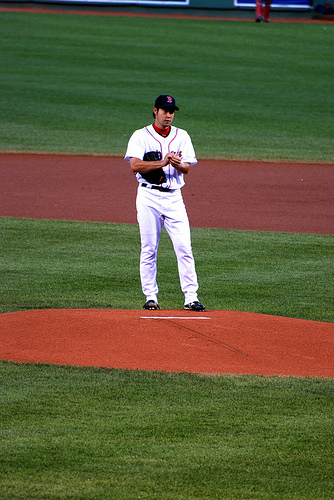
\includegraphics[height=3.65cm]{baseball_2410492.jpg}\\[-0.3em]
  {\scriptsize (a) 同图 target presence：球裤存在，机车不存在。}
\end{minipage}\hfill
\begin{minipage}[t]{0.375\textwidth}
  \centering
  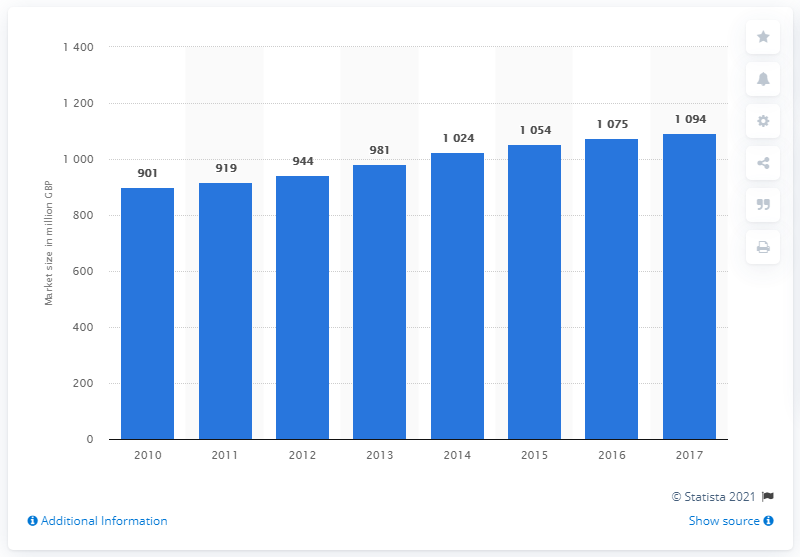
\includegraphics[width=\linewidth]{chart_2017.png}\\[-0.3em]
  {\scriptsize (b) 固定 target“最高柱及年份”，正确 value 为 2017。}
\end{minipage}\hfill
\begin{minipage}[t]{0.375\textwidth}
  \centering
  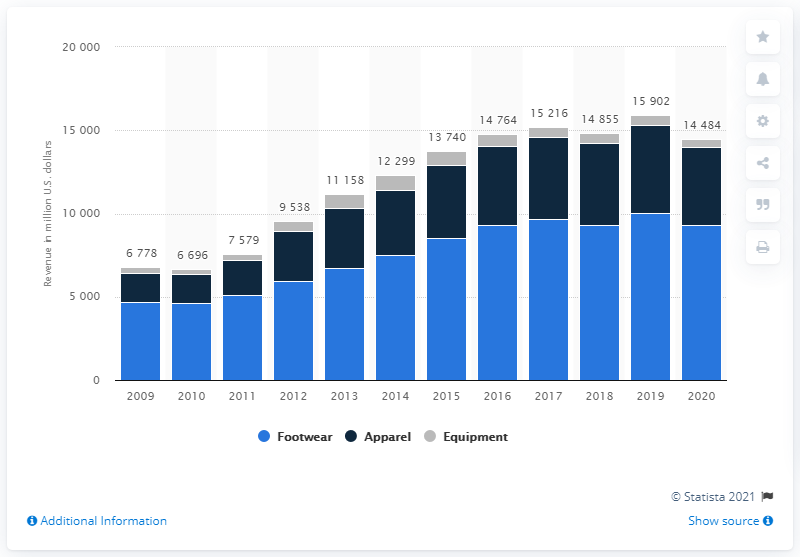
\includegraphics[width=\linewidth]{chart_2019.png}\\[-0.3em]
  {\scriptsize (c) 同一 target 在另一图中应翻转为 2019。}
\end{minipage}
\caption{Audited grounding 的实际样例。图 (a) 对同一视觉输入使用正/负 target；图 (b)(c) 固定 query/target，只要求 $D$ 随图像携带不同 value。图片仅用于解释已执行测试，不扩充 evaluation population。}
\label{fig:examples}
\end{figure*}

\subsection{五个 checkpoint}
为简洁起见，C-T1 表示 Balanced $T=1$/contextual/full D-DeepStack；E-T1 把 provider 改为 target-token embedding；C-Legacy 使用 summed-NLL；C-Main 关闭学习到的 D-DeepStack；C-T0.1 只把 Balanced temperature 改为 0.1。

\begin{table*}[t]
\centering
\caption{同分布 target specificity 与 evidence readability。Top-1/MRR 越高越好；gap 与 wrong-same advantage 越大表示 correct $D$ 和同图错误 $D$ 分离越强；correct-$D$ NLL 越低越好。}
\label{tab:retrieval}
\small
\begin{tabular}{lrrrrr}
\toprule
Checkpoint & Top-1 & MRR & Mean gap & Correct-$D$ NLL & Wrong-same win / advantage \\
\midrule
\textbf{C-T1} & 82.5\% & 0.906 & \textbf{2.431} & 1.286 & 93.5\% / \textbf{4.643} \\
E-T1 & 70.5\% & 0.833 & 0.773 & 1.292 & 86.0\% / 2.113 \\
C-Legacy & \textbf{86.0\%} & \textbf{0.925} & 0.308 & 1.376 & 94.0\% / 0.571 \\
C-Main & 50.0\% & 0.701 & 0.053 & 1.293 & 74.5\% / 0.234 \\
C-T0.1 & 85.5\% & 0.919 & 0.419 & \textbf{1.260} & \textbf{94.5\%} / 0.748 \\
\bottomrule
\end{tabular}
\end{table*}

\begin{table}[!t]
\centering
\caption{Audited causal grounding。Cross/target continuation 分母分别为 18/72；所有 healthy termination 均不低于 70/72。Presence separation 大于 0 才是期望方向。}
\label{tab:grounding}
\scriptsize
\resizebox{\columnwidth}{!}{%
\begin{tabular}{lrrrr}
\toprule
Checkpoint & Cross flip & Cross continuation & Presence separation & Target continuation \\
\midrule
\textbf{C-T1} & \textbf{5/9} & 10/18 & \textbf{+0.407} & \textbf{39/72} \\
E-T1 & 2/9 & 9/18 & $-2.283$ & 10/72 \\
C-Legacy & 1/9 & 5/18 & $-0.968$ & 4/72 \\
C-Main & \textbf{5/9} & \textbf{11/18} & \textbf{+0.958} & 6/72 \\
C-T0.1 & 1/9 & 6/18 & $-1.600$ & 27/72 \\
\bottomrule
\end{tabular}
}
\end{table}

\subsection{结果解释}
\paragraph{Contextual conditioning 是必要证据。}
C-T1 相对 E-T1 将 Top-1 从 70.5\% 提升至 82.5\%，mean gap 从 0.773 提升至 2.431，presence separation 从 $-2.283$ 翻转到 $+0.407$。两者 correct-$D$ NLL 接近，说明差异主要不是 evidence 的一般语言可读性，而是 target condition 是否携带足够的上下文语义。

\paragraph{Balanced $T=1$ 比单看排名更可靠。}
C-Legacy 与 C-T0.1 的 Top-1 分别为 86.0\% 和 85.5\%，表面上高于 C-T1；但其 mean gap 只有 0.308/0.419，cross flip 仅 1/9，presence separation 均为负。Top-1 只要求 correct cell 略胜，无法反映 margin、因果翻转或不存在 target 的错误注入。Balanced $T=1$ 因而保留为默认，而非追逐单一 retrieval accuracy。

\paragraph{D-DeepStack 承载丰富语义。}
C-Main 在简单 presence separation（$+0.958$）与 cross flip（5/9）上不差，说明主 $D$ 可以表达某些粗粒度存在性；然而其 Top-1 降到随机附近的 50.0\%，mean gap 为 0.053，target continuation 仅 6/72。完整 D-DeepStack 不是装饰性旁路，而是同图 target discrimination 与具体 evidence readout 的主要组成。

\paragraph{Norm 不是质量代理。}
五个 checkpoint 均无 token-collapse warning。C-T1 的 main $D$/source mean norm ratio 为 1.265，三个分支为 2.342/2.706/2.020；C-Legacy 的三个分支升至 4.155/4.132/2.568，却没有带来 grounding 优势。因此当前 Norm 只作为训练稳定性与尺度健康项，不能被解释为 target specificity 指标，也没有证据支持增加更多 norm 模式。

\section{Hallucination：当前发现与局限}
Target hallucination 是本项目和潜在审稿中最关键的问题之一：若图中不存在 $z$，但 Adapter 仍根据 target 文本生成看似匹配的 $D$，工具就从“视觉证据提取器”退化为“target 条件生成器”。当前证据既发现了这一风险，也暴露了评测本身尚不成熟。

图~\ref{fig:examples}(a) 是最直接的失败例。对 C-T1，正 target“球裤区域”在 free continuation 中输出 PRESENT；但负 target“机车车体”也输出 PRESENT，并生成“locomotive body and side panels are visible”的虚假描述。这个单例明确证明：最佳 checkpoint 仍会发生 target hallucination，平均指标不能掩盖它。

同时，teacher-forced log-odds 与自由生成并不总一致。该负 target 的 $r^-$ 仍为负，但 greedy continuation 却输出 PRESENT。五个 checkpoint 的绝对 \code{actual\_direction\_accuracy} 与 \code{negative\_false\_positive\_rate} 都被强烈标签先验压成 0，尽管 pairwise separation、自由生成和人工观察显示显著差异。因此本文使用 $r^+-r^-$ 作相对诊断，但不把零阈值指标当作有效结论。

当前验证还有以下限制：
\begin{enumerate}
  \item 只有 36 个 same-image presence pairs 与 9 个 cross-image pairs，覆盖面、置信区间和随机种子都不足；
  \item negative target 由人工构造且通常语义差异很大，未系统匹配长度、词频、视觉类别、局部位置和 hard-negative 难度；
  \item PRESENT/NOT\_PRESENT 的 base-model label prior 未校准，严格字符串抽取会混合 grounding、格式遵循和 OCR/生成错误；
  \item teacher-forced mean token log-prob、greedy continuation 与真正的 tool-use downstream behavior 不是同一测量对象；
  \item pair 由开发阶段人工审计，没有独立 blind annotation、inter-annotator agreement 或外部 benchmark protocol；
  \item 同一个冻结 8B reader 既定义训练可读性又参与评测，尚不能排除 reader-specific co-adaptation。
\end{enumerate}

因此，这套 audited diagnostics 的适当定位是\textbf{轻量、初步、用于发现失败和筛选 checkpoint}。它不是规范 hallucination benchmark，也不能支持“方法解决了 hallucination”的论文主张。后续应单独设计更大、更难、盲审且经过 calibration 的 target-existence/target-content benchmark，并明确区分视觉不存在、属性错误、关系错误、位置错误和 target-text leakage；还应联合报告 teacher-forced intervention、自由生成与最终任务行为。该工作很重要，但不在本报告阶段执行，也不在此处提前冻结具体方案。

\section{正确性证据与可复现性}
当前实现的主要 correctness gates 包括：
\begin{itemize}
  \item 原生 Qwen transcript round trip、无 tokenizer growth、无重复 think opener；
  \item target span、canonical/model token mapping 与 contextual $H_z$ identity；
  \item 两种 conditioning providers 经过同一 typed Adapter boundary；
  \item Matrix-CE 的 length balance、legacy 保真和 streaming/manual-gradient 对 autograd parity；
  \item main $D$ 与所有 D-DeepStack 分支作为同一 observation 原子交换；
  \item evidence queries 屏蔽原图 keys，correct/wrong/random/no-$D$ 控制共享同一 token/mask contract；
  \item 两卡 FSDP2 accumulation、global numerator/count reduction、checkpoint teardown/resume 与 Adapter-only export；
  \item artifact、数据、prompt、processor、provider、branch layout 和 projection identity 的严格绑定。
\end{itemize}

\begin{table}[!t]
\centering
\caption{五份 immutable internal-evaluation report。SHA256 为报告文件 hash；checkpoint identity 为 artifact manifest identity；表中均作首尾缩写。}
\label{tab:artifacts}
\scriptsize
\setlength{\tabcolsep}{2pt}
\begin{tabularx}{\columnwidth}{l l l Y}
\toprule
ID & Checkpoint identity & Report SHA256 & 主要变量 \\
\midrule
C-T1 & \code{dfa992fc...e10} & \code{4fcd6faa...704} & contextual, Balanced $T=1$, full DS \\
E-T1 & \code{3cccf99e...469} & \code{af6b5d2f...9e3} & target embedding, Balanced $T=1$, full DS \\
C-Legacy & \code{bc5b78c2...5b7f} & \code{7308f053...6bb} & contextual, summed-NLL, full DS \\
C-Main & \code{c80c616c...fc8b} & \code{54674da3...492} & contextual, Balanced $T=1$, main $D$ only \\
C-T0.1 & \code{3ff14e66...f49e} & \code{02e299f3...baa} & contextual, Balanced $T=0.1$, full DS \\
\bottomrule
\end{tabularx}
\end{table}

五份 report 共享 data-manifest identity \code{534f5b1e...6b0}、model identity \code{73334646...57c}、prompt hash \code{bf085a6e...3c9}、seed 42，以及 grounding manifest file SHA256 \code{a65aa6e6...8c0}。图像 provenance 与原始文件 hash 记录在 \path{reports/figures/PROVENANCE.md}。

\section{结论}
当前 representation phase 已形成一条闭合的原生 Qwen 训练路径：从 tool-call target span 提取 $H_z$，以双向 target--vision attention 调制主视觉与三个 DeepStack 分支，经冻结 Qwen merger 生成完整 latent observation，再用同图 Matrix CE 约束 target specificity、用 $L_{\mathrm{gen}}$ 约束因果可读性。训练不扩展 tokenizer、不更新 Qwen，也不借用历史 checkpoint 初始化。

五个 2,000-step checkpoint 的统一比较支持三项选择：contextual hidden state 优于 target-token embedding；Balanced $T=1$ 优于 legacy summed-NLL 和 $T=0.1$ 的表面高 Top-1；完整 D-DeepStack 对丰富 target-specific evidence 必不可少。因此 C-T1 是当前进入 policy RL phase 的 representation artifact 选择。

该选择不是 hallucination 问题的终点。最佳 checkpoint 仍在清晰不存在的 target 上生成虚假证据；现有 36+9 pair 测试又过小且存在 label-prior 与测量不一致。最准确的结论是：当前方法已经证明 $D$ 可读、同图可分，并取得有限的 causal grounding evidence，但尚未证明对不存在 target 的稳健拒绝。后续独立 hallucination study 是进入更强方法主张前的必要工作。

\end{document}
